% Source: graduate-coursework/Research/Intro_to_Agents/handouts/Part2_Agent_Foundations.tex

\documentclass[border=4pt]{standalone}
\usepackage{amsmath}
\usepackage{amssymb}
\usepackage{tikz}
\usepackage{xcolor}
\usetikzlibrary{shapes.geometric, arrows.meta, positioning, fit, calc, backgrounds}

\definecolor{UofSCGarnet}{HTML}{73000a}
\definecolor{UofSCBlack}{HTML}{000000}
\definecolor{UofSCWhite}{HTML}{ffffff}
\definecolor{UofSCAtlantic}{HTML}{466A9F}
\definecolor{UofSCCongaree}{HTML}{1F414D}
\definecolor{UofSCRose}{HTML}{CC2E40}
\definecolor{UofSCHorseshoe}{HTML}{65780B}
\definecolor{UofSCGrass}{HTML}{CED318}
\definecolor{UofSCHoneycomb}{HTML}{A49137}
\definecolor{UofSCDarkGarnet}{HTML}{570008}
\definecolor{UofSCAzalea}{HTML}{844247}
\definecolor{UofSC90Black}{HTML}{363636}
\definecolor{UofSC70Black}{HTML}{5C5C5C}
\definecolor{UofSC50Black}{HTML}{A2A2A2}
\definecolor{UofSCWarmGrey}{HTML}{676156}
\definecolor{UofSCSandstorm}{HTML}{FFF2E3}

\tikzset{
    % Box styles with sharp corners
    component/.style={
        rectangle,
        draw=UofSCBlack,
        fill=UofSCWhite,
        thick,
        minimum width=3cm,
        minimum height=1cm,
        align=center,
        font=\small
    },
    component garnet/.style={
        component,
        fill=UofSCGarnet!10,
        draw=UofSCGarnet,
        thick
    },
    component atlantic/.style={
        component,
        fill=UofSCAtlantic!10,
        draw=UofSCAtlantic,
        thick
    },
    component congaree/.style={
        component,
        fill=UofSCCongaree!10,
        draw=UofSCCongaree,
        thick
    },
    loop node/.style={
        rectangle,
        draw=UofSCGarnet,
        fill=UofSCGarnet!15,
        thick,
        minimum width=2.5cm,
        minimum height=1.2cm,
        align=center,
        font=\footnotesize\bfseries
    },
    decision/.style={
        diamond,
        draw=UofSCBlack,
        fill=UofSCHoneycomb!20,
        thick,
        minimum width=2cm,
        minimum height=1.5cm,
        align=center,
        font=\footnotesize,
        aspect=2
    },
    arrow style/.style={
        ->,
        >=Stealth,
        thick,
        UofSCBlack
    },
    biarrow style/.style={
        <->,
        >=Stealth,
        thick,
        UofSCBlack
    }
}

\begin{document}
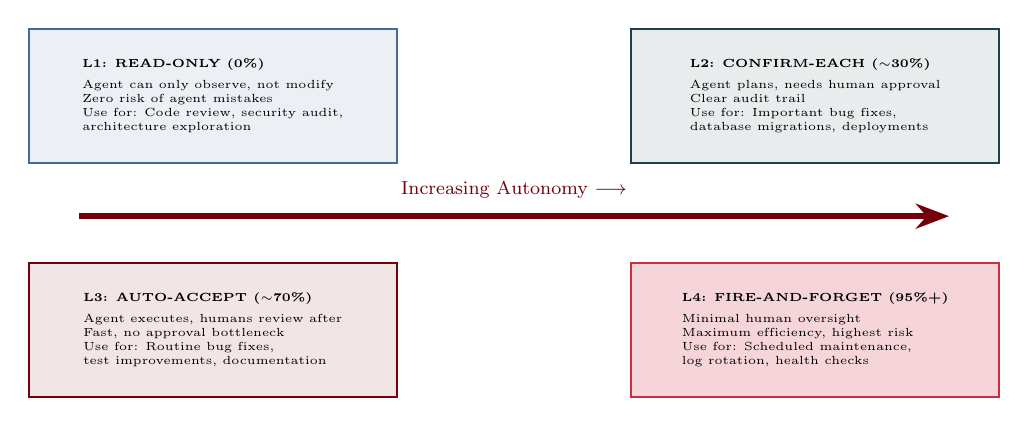
\begin{tikzpicture}[scale=0.85, transform shape]
        % L1
        \node[component atlantic, minimum width=5.5cm, minimum height=2cm, align=left, font=\tiny] (l1) at (-4.5, 2) {
            \textbf{L1: READ-ONLY (0\%)}\\[0.1cm]
            Agent can only observe, not modify\\
            Zero risk of agent mistakes\\
            Use for: Code review, security audit,\\
            architecture exploration
        };

        % L2
        \node[component congaree, minimum width=5.5cm, minimum height=2cm, align=left, font=\tiny] (l2) at (4.5, 2) {
            \textbf{L2: CONFIRM-EACH ($\sim$30\%)}\\[0.1cm]
            Agent plans, needs human approval\\
            Clear audit trail\\
            Use for: Important bug fixes,\\
            database migrations, deployments
        };

        % L3
        \node[component garnet, minimum width=5.5cm, minimum height=2cm, align=left, font=\tiny] (l3) at (-4.5, -1.5) {
            \textbf{L3: AUTO-ACCEPT ($\sim$70\%)}\\[0.1cm]
            Agent executes, humans review after\\
            Fast, no approval bottleneck\\
            Use for: Routine bug fixes,\\
            test improvements, documentation
        };

        % L4
        \node[component, fill=UofSCRose!20, draw=UofSCRose, minimum width=5.5cm, minimum height=2cm, align=left, font=\tiny] (l4) at (4.5, -1.5) {
            \textbf{L4: FIRE-AND-FORGET (95\%+)}\\[0.1cm]
            Minimal human oversight\\
            Maximum efficiency, highest risk\\
            Use for: Scheduled maintenance,\\
            log rotation, health checks
        };

        % Arrow showing progression
        \draw[arrow style, line width=2pt, UofSCGarnet] (-6.5, 0.2) -- (6.5, 0.2);
        \node[font=\footnotesize, text=UofSCGarnet] at (0, 0.6) {Increasing Autonomy $\longrightarrow$};
    \end{tikzpicture}
\end{document}
